\chapter{Consumer Theory}

Choice theory says that a rational decision-maker picks the most
preferred option from her choice set. Consumer theory specializes this
framework to the most extensively studied application — a consumer
choosing bundles of goods subject to a budget constraint — and uses the
\emph{preference-based approach} throughout. The agenda has three parts:

\begin{enumerate}

\item
  \textbf{Formalize the choice set and preferences.}
  \begin{itemize}
  \item
    Set of alternatives: the \emph{consumption set}.
  \item
    Choice set (within the consumption set): the \emph{budget set}.
  \item
    Preferences: a \emph{utility representation} of the preference
    relation.
  \end{itemize}
\item
  \textbf{Derive optimal choices} from the budget set and the preference
  relation.
\item
  \textbf{Analyze the properties} of those optimal choices — i.e., of
  demand.
\end{enumerate}

\section{Setups}\label{setups}

We start with four assumptions that we will maintain throughout consumer
theory:
\asm{}{
\begin{enumerate}

\item
  \emph{Perfect} information.
\item
  Consumers are \emph{price takers}.
\item
  Prices are \emph{linear}.
\item
  Goods are \textit{divisible}.
\end{enumerate}
}

\rmkb{
\begin{itemize}
    \item \emph{Price-taking} means the consumer treats prices \(\p\) as known, fixed, and exogenous — no searching for deals, no bargaining for discounts.
    \item \emph{Linear prices} means the total cost of a bundle is just \(\p\cdot\x\); no quantity discounts or two-part tariffs.
    \item \emph{Divisibility} is captured by working in \(\RR_+^n\). This is mostly a mathematical convenience: a discrete-good problem can still be analyzed by restricting attention to the integer points in \(\RR_+^n\), so the divisibility assumption does not rule out applications to indivisible goods.
\end{itemize}
}

For simplicity, we take the consumption set to be the entire non-negative orthant.

\defn{Consumption Set}{
With \(n\) goods, the \textit{consumption set} is given by:
\[X = \RR_+^n = \{\x \in \RR^n: x_i\ge 0 \text{ for } i  = 1,2,\cdots,n \}.\]
}

The budget set is a subset of the consumption set; it further restricts the bundles the consumer can actually afford given income and prices.

\defn{Budget Set}{
With \(n\) goods and income of \(m\), given a price vector
\(\p  =(p_1,\cdots,p_n)'\ge 0,\p\ne \bold 0\), the \textit{budget set} is given by:
\[B(\p,m) = \{\x\in\RR^n: \p\cdot\x\le m,\x\ge\0 \}.\]
}

\rmk{
By reinterpreting the consumption goods and the
budget, the derivation of the budget set can be extended to
encompass other economic problems. For example, consumption-leisure
choice, and inter-temporal choice.
}

\section{Utility Representation}\label{utility-representation}

Preference relations are intuitive but awkward to work with directly.
A utility representation lets us recast preference maximization as
ordinary optimization over a real-valued function — a much more
tractable object.

\defn{Utility Representation}{
A preference relation \(\pref\) on \(X\)
is represented by a \textit{utility function} \(u:X\to \RR\) if
\[x\pref y \iff u(x)\ge u(y).\]
}

This definition makes utility an \emph{ordinal} object: the actual
numerical values carry no economic content. Only the implied ranking
matters — \(u\) encodes the consumer's relative preferences over
bundles, nothing more.

If \(u\) represents \(\pref\), then the choice rule defined upon budget
set is:
\[C(B(\p,m);\pref) = \left\{\x\ | \ \x \text{ solves }\max_{\x\in B(\p,m) } u(\x) \right\}.\]


\rmk{
An equivalent notation of such choice rule is
\(C_\succeq(B)\).
}

The natural question is whether \emph{every} rational preference relation
admits a utility representation. If the consumption set \(X\) is
\textit{finite}, the answer is yes — and the construction is direct.

\propp{}{
If \(X\) is finite, then any rational
(complete and transitive) preference relation \(\pref\) on \(X\) can be
represented by a utility function \(u:X\to \{1,\cdots,n\}\), where
\(n = |X|\).
}{
Proceed by induction on \(|X|\).
\begin{itemize}
\item
  \emph{Base case:} \(|X| = 1\), say \(X = \{x\}\). Set \(u(x) = 1\).
  The condition holds vacuously.
\item
  \emph{Inductive step:} suppose any rational preference on a set of
  size \(n\) admits the desired representation. Take any \(X\) with
  \(|X| = n+1\).

  \begin{itemize}
  \item
    Since \(C_{\pref}(X)\) is non-empty (Ch.~1 Proposition on finite
    choice sets), the complement \(Y = X\setminus C_\pref(X)\) has at
    most \(n\) elements. By the inductive hypothesis, the restriction of
    \(\pref\) to \(Y\) admits a utility representation
    \(u: Y\to \{1,2,\ldots,n\}\).
  \item
    We extend the domain of \(u\) to \(X\) by setting \(u(x) = n+1\) for
    each \(x \in C_\pref (X)\). By construction, we have
    \(u(x) \in \{1,\cdots, n,n+1\}\) for all \(x\in X\).
  \item
    Now we show that the constructed \(u\) represents \(\pref\), i.e.,
    for any \(x,y\in X\), \(x\pref y\) if and only if
    \(u (x) \ge u(y)\). Suppose \(x\pref y\). There are three
    possibilities:

    \begin{itemize}
    \item
      \(x\in C_\pref(X),y\in Y\)\(\iff\) \(u(x) = n+1 \ge u(y)\).
    \item
      \(x,y\in C_\pref(X)\) \(\iff\) \(u(x) = u(y) = n+1\), also,
      \(u(x)\ge u(y)\).
    \item
      \(x,y\in Y\). Then, since by construction \(u\) represents
      \(\pref\) on \(Y\), \(x\pref y \) if and only if \(u(x)\ge u(y)\).
    \end{itemize}
  \end{itemize}
\end{itemize}
}

When \(X\) is infinite the situation is more subtle. In general, a
rational preference relation on \(\RR_+^n\) need not admit a utility
representation \(u:\RR_+^n\to \RR\). The standard counter-example is
lexicographic preferences.

\ex{
Consider the
lexicographic preferences on the square \(X = \RR^2\), where 
\((x_1,x_2)\succ (y_1,y_2)\) if either (1) \(x_1>y_1\) or (2)
\(x_1 = y_1\) and \(x_2 > y_2\). These preferences cannot be represented
by a utility function, and this is also an example for which
``indifference curves" do not exist, because the agent is never
indifferent between any two choices.

To see this, suppose by contradiction there exists a utility
representation \(u(x,y)\). For any \(x\in \RR_+\), consider the interval
\(I(x) = \left(\inf_y u(x,y), \sup_y u(x,y) \right)\). \(I(x)\) is not
degenerate, and \(I(x_1),I(x_2)\) do not overlap for \(x_1\ne x_2\).
Since rational numbers are dense, we construct a function $r$ to pick a rational number inside $I(x)$, i.e., \(r(x)\in I(x)\). Since \(I(x_1),I(x_2)\) do not overlap,
\(r(x_1)\ne r(x_2)\) for \(x_1\ne x_2\). Thus, \(r:\RR_+\to \QQ_+\) is an injective function. Since \(\RR_+\) is uncountable and \(\QQ_+\) is
countable, this mapping is impossible.

However, note that if we replace \(X = \RR_+^2\) with \(X' = \QQ_+^2\),
the lexicographic preference relation would admit a utility
representation. More generally, this idea is formalized into the
proposition in countable set case.
}

For \emph{countable} \(X\) (possibly infinite), every rational
preference relation admits a utility representation — and the
construction below gives one explicitly.

\propp{}{
If \(X\ne\varnothing\) is countable, then any
rational (complete and transitive) preference relation \(\pref\) on
\(X\) can be represented by a utility function \(u:X\to (0,1)\).
}{
\begin{itemize}
\item
  First, construct a mapping of utility function \(u:X\to (0,1)\).

  \begin{itemize}
  \item
    Let \((x_n)_{n = 1}^\infty\) be a countable enumeration of \(X\).
  \item
    Let \(u(x_1) = \frac12\). Consider \(x_{n+1}\), \(n\ge 1\).

    \begin{itemize}
    \item
      If \(x_{n+1}\sim x_i\) for some \(1\le i\le n\), then define
      \(u(x_{n+1}) = u(x_i)\).
    \item
      Otherwise, define
      $$
\begin{aligned}
      M_n &= \max\{\max\{u(x_i): x_{n+1}\succ x_i,1\le i\le n \},0 \}\\
      m_n  &= \min\{\min\{u(x_i): x_{i}\succ x_{n+1},1\le i\le n \},1 \}\\
      \end{aligned}
$$

      By construction \(M_n>m_n\). Define
      \(u(x_{n+1}) = \frac{M_n + m_n}2\).
    \end{itemize}
  \end{itemize}
\item
  Second, prove that \(u(\cdot)\) is a utility representation of
  preference relation \(\pref\).

  \begin{itemize}
  \item
    Take any \(y,z\in X\). Since \(X\) is countable, \(\exists i,j\)
    such that \(y = x_i\) and \(z = x_j\). Without loss of generality,
    suppose \(i\le j\).
  \item
    By construction, \(u(x_i) = u(x_j)\) if and only if \(x_i\sim x_j\).
    For \(x_j \nsim x_i\), \(u(x_j)>u(x_i)\) if and only if
    \(x_j\succ x_i\).
  \end{itemize}
\end{itemize}
}

The pathology of the lexicographic preference relation is a sudden
preference reversal: \((3,3)\succ (3,2)\), yet \((3,2)\succ (x,3)\)
for any \(x\) strictly less than \(3\) — the ranking jumps
discontinuously as \(x\) crosses \(3\). To rule this out we impose a
\emph{continuity} restriction on preferences. Continuity is also
desirable from a revealed-preference standpoint: any finite set of
observed choices that is consistent with HARP can be rationalized by
a continuous preference relation, so continuity costs us nothing
empirically.

\defn{Continuity}{
A preference relation \(\pref\) on
\(X\se \RR^n\) is \emph{{continuous}} if for any sequence
\(\{(x^n,y^n)\}_{n = 1}^\infty\) with \(x^n\to x,y^n\to y\), and
\(x^n\pref y^n\) for all \(n\), we have \(x\pref y\).
}

Continuity gives us more than mere existence of a utility
representation — it gives us a \emph{continuous} one.

\propp{}{
Any complete, transitive and continuous
preference relation \(\pref\) on \(X\) on \(X\se \RR^n\) can be
represented by a continuous utility function \(u:X\to \RR\).
}{
In order to have a simple, constructive proof, we prove the proposition
only for the case of a monotone preference relation \(\pref\) on
\(X = \RR_+^n\).

Let \(e = (1,\cdots,1)\) and consider bundles of the form
\(\alpha e = (\alpha,\cdots,\alpha)\) where \(\alpha \ge 0\). For each
\(x\in \RR_+^n\), we construct a utility number as follows:
\(u(x) = \max A(x)\), where
\(A(x) = \{\alpha\in R_+:\alpha e \preceq x\}\). To see that the set
\(A(x)\) has a maximal point, note that the set is

\begin{itemize}
\item
  Nonempty, since \(0 \in A(x)\) by monotonicity of \(\pref\);
\item
  Closed, by the continuity of \(\pref\);
\item
  Bounded, since by monotonicity of \(\pref\),
  \(\alpha \le \max \{x_1,\cdots,x_n\}\) for each \(\alpha \in A(x)\).
\end{itemize}

Now we show that we must have \(u(x)e\sim x\).

\begin{enumerate}

\item
  \(u(x)e\preceq x\). This is satisfied by construction of
  \(u(x)\in A(x)\).
\item
  \(u(x)e\pref x\). For each \(n\ge 1\), we have
  \(u(x)+\frac1n \notin A(x)\), hence \((u(x) + \frac1n)e\npreceq x\),
  therefore by completeness of \(\pref\) we have
  \((u(x)+\frac1n)e\pref x\), which by continuity of \(\pref\) implies
  \[\lim\limits _{n\to \infty} (u(x)+\frac1n)e = u(x)e\pref x.\]
\end{enumerate}

Now it remains to show that the constructed utility function
\(u(\cdot)\) has

\begin{enumerate}

\item
  Ability to represent the preference relation \(\pref\), and
\item
  Continuity.
\end{enumerate}

For representation part, note that by transitivity \(x\pref y\) if and
only if \(u(x)e\pref u(y)e\) (since \(u(x)e\sim x\pref y \sim u(y)e\)),
and by monotonicity of \(\pref\), this holds if and only if
\(u(x) \ge u(y)\). For continuity part, this is more subtle and not
covered here.
}

\rmkb{
\begin{enumerate}

\item
  The construction in the proof specifies the utility of any bundle
  \(x\) by finding the point on the 45° line on the indifference curve
  passing through \(x\).

  \begin{itemize}
  \item
    This specification is, of course, completely arbitrary; just for
    mathematical convenience.
  \item
    To reflect this arbitrariness, utility representation of preferences
    is \emph{ordinal}, i.e., only the induced preference ordering of
    choices is meaningful, instead of the exact utility numbers assigned to
    them.
  \item
    In fact, if \(u\) represents \(\pref\), then
    \(U(\cdot) = v(u(\cdot))\) also represents \(\pref\) so long as
    \(v:\RR\to \RR\) is an increasing function.
  \end{itemize}
\item
  The thought process and the introduction of the additional assumption
  are the most important for this part.

  \begin{itemize}
  \item
    Recall that our motivation is to come up with a tractable framework
    to analyze the consumer's problem. One possibility
    is to attach a utility level to each consumption bundle (ordinal
    utility representation).
  \item
    We ask whether any preference relation can be represented by a
    utility function. The answer is yes, if the consumption set \(X\) is
    finite (or countable), but no if \(X = \RR_+^n\). We notice that the
    problem with the counter-example (e.g., the lexicographic preference
    relation) is that there are sudden preference reversals.
  \item
    We then impose the restriction of ``continuity" of preferences to
    rule out those unfavorable scenarios and show that any
    rational and continuous preference relation on \(X = \RR_+^n\) can be
    represented by a continuous utility function.
  \end{itemize}
\item
  The continuity of preference relation and continuity of its utility
  representation is not interdependent. If a preference relation can be
  represented by a continuous utility function, then such preference
  relation must be continuous. On the other hand, a continuous
  preference relation can be represented by a discontinuous utility
  function, if you like. (That is not convenient for
  mathematical issues though.)
\end{enumerate}
}

\section{Utility Maximizing Problem}\label{utility-maximizing-problem}

What distinguishes consumer theory from the general choice-theoretic
framework is the specific structure of the consumer's choice set —
it is determined by prices and wealth. This structure is what lets us
derive economically meaningful comparative statics. With a utility
representation \(u(\cdot)\) of \(\pref\) in hand, the consumer's
optimization is the \emph{Utility Maximization Problem} (UMP), also
called the \emph{Consumer Problem} (CP).

\defn{Utility Maximization Problem}{
$$
\begin{aligned}
& \max_{\x\in \RR_+^n} u(\x)\\
\text{s.t. }& \p\cdot \x\le m\\
& x_i\ge 0,\forall i = 1,2,\cdots,n
\end{aligned}
$$
}

That is: given prices \(\p = (p_1,\ldots,p_n)'\ge \0,\;\p\ne\0\) and
wealth \(m\), the consumer picks a non-negative bundle
\(\x = (x_1,\ldots,x_n)'\) to maximize utility subject to spending no
more than \(m\). Equivalently, the CP can be written as:
\[C(B(\p,m);\pref) = \left\{\x\ \bigg| \ \x \text{ solves }\max_{\y\in B(\p,m) } u(\y) \right\}.\]

\subsection{Existence of Optimal Choice(s)}\label{existence-of-optimal-choices}

The first question is whether the UMP has any solution. Under mild
conditions, it does.

\propp{}{
Suppose that the consumer has a rational
(complete and transitive) and continuous preference relation and makes
rational decisions, then for \((\p,m)\gg \0\), they have (at least) one
optimal choice.
}{
\begin{itemize}
\item
  Since the consumer has a complete, transitive and continuous
  preference relation, then her preferences can be represented by a
  continuous utility function \(u(\cdot)\).
\item
  When \((\p,m)\gg \0\), the budget set \(B(\p,m)\) is closed and
  bounded and hence compact.
\item
  A continuous function on a compact set has at least one maximizer.
\end{itemize}
}

\subsection{Further Assumptions}\label{further-assumptions}

Existence is guaranteed under rationality, continuity, and
\((\p,m)\gg\0\). The remaining questions are practical:

\begin{itemize}
\item How do we actually \emph{find} the optimal choice(s)?
\item Which additional restrictions on \(\pref\) simplify the analysis?
\end{itemize}

\paragraph{Locally Non-Satiation}\label{locally-non-satiation}

One useful simplification is to replace the budget inequality with the
equality \(\p\cdot \x = m\). Intuitively, if the consumer always thinks
``more is better,'' she should never leave money on the table — at any
optimum, she exhausts her budget.

\defn{Monotonicity}{
A preference relation
\(\pref\) on \(X = \RR_+^n\) is \emph{{monotone}} if for any
\(\x,\y\in X\), we have:

\begin{itemize}
\item
  \(\x \ge \y\too \x \pref\y\);
\item
  \(\x \gg \y\too \x \succ \y\).
\end{itemize}
}

Monotonicity is more than we need; the weaker condition of
\emph{local non-satiation} already does the job.

\defn{Locally Non-Satiation}{
A preference relation
\(\pref\) on \(X = \RR_+^n\) is \emph{{locally non-satiated}} if
for any \(\x\in X\) and \(\varepsilon >0\), there exists
\(\y \in Ball(\x,\varepsilon)\cap X\) such that \(\y\succ \x\).
}

Intuitively, local non-satiation rules out any \emph{bliss point}: from
any bundle, the consumer can do strictly better with an arbitrarily
small change. Note that monotonicity implies local non-satiation (but
not conversely).

\propp{}{
Suppose that the consumer has a complete,
transitive, continuous and locally non-satiated preference relation and
makes rational decisions, then for \((\p,m)\gg \0\), the budget
constraint must hold with equality at any optimal choice \(\x^*\), i.e.,
\(\p\cdot \x^* = m\).
}{
Intuitively, if the consumer does not exhaust her budget, then there
must be a nearby affordable bundle which is strictly more preferred, by
locally non-satiation.

\begin{itemize}
\item
  Consider any bundle \(\x \in X = \RR_+^n\) where \(\p\cdot\x<m\). Since
  the preference relation \(\pref\) is locally non-satiated, for any
  \(\varepsilon >0\), there exists
  \(\y \in Ball(\x,\varepsilon) \cap X\) such that \(\y\succ \x\).
\item
  We claim that \(\y \in B(\p,m)\), i.e., the alternative bundle falls within the consumer's
  budget set for \(\varepsilon > 0\) small enough, so that \(\x\)
  cannot be an optimal choice.

  Let \(\y = \x + \z\). By construction, \(||\z||< \varepsilon\). In
    particular, \(|z_i|<\varepsilon\), for any \(i = 1,2,\cdots,n\). It
    follows that
    \(\p\cdot \y = \p \cdot \x + \p \cdot \z \le \p\cdot\x + n\cdot \varepsilon\cdot \max_i p_i\).
    As \(\varepsilon\) take appropriately small values, we finish our
    proof.
\end{itemize}
}

\paragraph{Convexity}\label{strict-convexity}

Another possible simplification is the case of \emph{unique} optimal
choice. Notice that the consumer's budget set
\(B(\p,m)\) is convex. Based on this, when the utility function
\(u(\cdot)\) is \emph{strictly quasi-concave}, there is a \emph{unique}
global maximizer. This translates into the following condition of
strictly convex preference relations.

\defn{Convexity}{
A preference relation \(\pref\) on
\(X = \RR_+^n\) is \emph{convex} if for any \(\x,\y,\z\in X\) such that
\(\x \pref \z\) and \(\y \pref \z\), we have \(t\x+ (1-t)\y\pref\z\),
for any \(t\in [0,1]\). If \(t\x + (1-t)\y \succ \z\) for any
\(\x \ne \y\) and \(t\in (0,1)\), then the preference relation is
\emph{strictly convex}.
}

\rmkb{
\begin{enumerate}
\item
  Convexity can be equivalently defined as: For any \(\x,\y\in X\) such
  that \(\y\pref \x\), we have \(t\y + (1-t)\x\pref \x\) for any
  \(t\in [0,1]\).
\item
  An equivalent way to describe convexity involves indifference curve
  and \emph{upper contour set} of choice bundles, 
  \(\text{Upper Contour Set of }y = \{x\in X: x\pref y\}\), graphically
  the area sitting upper-right above the indifference curve (included).
  Convexity of preferences amounts to the assumption that the upper
  contour set of any \(y\in X\), is a \emph{convex} set.
\item
  Convexity is fundamental in the standard model of competitive
  economics. When consumer preferences are convex, market
  clearing prices exist; otherwise this may not exist. Convexity is also
  needed to be able to recover consumer preferences from choices from
  various budget sets. Convexity is often described as capturing the
  idea that the agent like diversity. However, whether convexity makes
  sense often depends on the interpretation of the goods space, in
  particular on the level of aggregation (e.g., over time or
  categories).
\end{enumerate}
}

\propp{}{
Suppose that the consumer has a complete,
transitive, continuous and strictly convex preference relation and makes
rational decisions, then for \((\p,m)\gg\0\), there is exactly one
optimal choice.
}{
\begin{itemize}
\item The rational and continuous preference relation has guaranteed the
existence of at least one optimal choice. 
\item 
Suppose to the contrary that
the consumer has at least two optimal choices \(\x^*\) and \(\y^*\), and
\(\x^*\ne \y^*\), then by optimality \(\x^*\sim \y^*\). Construct a bundle \(\bold w = \frac12 \x^* + \frac12 \y^*\). Since the
consumer's preference relation is strictly convex, \(\w\succ \x^* \sim \y^*\). Moreover, since the budget set
\(B(\p,m)\) is convex when \((\p,m)\gg \0\), so \(\bold w \in B(\p,m)\).
So neither \(\x^*\) nor \(\y^*\) can be an optimal choice, which is a
contradiction.
\end{itemize}
}

These assumptions on \(\pref\) each have a direct counterpart on any
representing utility function \(u\). The translation makes it easier to
work in the utility space and import the right structural property
without re-deriving it.

\prop{}{
Suppose the preference relation \(\pref\) on
\(X\) can be represented by \(u:X\to \RR\). Then,

\begin{enumerate}
\item
  \(\pref\) is monotone if and only if \(u\) is non-decreasing.
\item
  \(\pref\) is locally non-satiated if and only if \(u\) has no local
  maxima in \(X\).
\item
  \(\pref\) is (strictly) convex if and only if \(u\) is (strictly)
  quasi-concave.
\end{enumerate}
}

\subsection{Marshallian Demand \& Indirect Utility Function}\label{marshallian-demand--indirect-utility-function}

\defn{Indirect Utility Function}{
Given $(\p,m)\gg \0$, the \emph{indirect utility function} is defined to give the optimal utility level:
\[v(\p,m) = \sup_{\x \in B(\p,m)} u(\x).\]
}

\rmk{
Here we rigorously use ``\(\sup\)" to define
\(v(\p,m)\) instead of ``\(\max\)", because sometimes \(u(\x)\) does not
behave well to have a maximum.
}

\defn{Marshallian Demand Correspondence}{
The \emph{Marshallian demand correspondence} is defined as the consumer's optimal choice(s):
\[\x^M(\p,m) = \left\{\x \in B(\p,m): u(\x) = v(\p,m) \right\}.\]
}
In general \(\x^M(\p,m)\) is a \emph{set} of utility-maximizing bundles
— it collapses to a single point only under strict convexity (see
below).

Throughout this section assume the consumer has a rational preference
relation \(\pref\) and faces \((\p,m)\gg\0\). The Marshallian demand
and indirect utility function inherit the following properties from
\(\pref\):

\prop{Properties of Marshallian Demand Correspondence and Indirect Utility Function}{
\begin{itemize}
\item
  \textbf{Existence of optimal choice(s)}: If \(\pref\) is continuous, then the
  Marshallian demand \(\x^M(\p,m)\ne \varnothing\).
\item
  \textbf{Structure of Marshallian demand}: If \(\pref\) is convex, then
  \(\x^M(\p,m)\) is a convex set. If \(\pref\) is strictly convex, then
  \(\x^M(\p,m)\) Is a singleton.
\item
  \textbf{Homogeneity}: Both \(v(\p,m)\) and \(\x^M(\p,m)\) are homogeneous of
  degree \(0\) in \((\p,m)\), that is, for any \(t>0\),
  \(v(t\p,tm) = v(\p,m)\) and \(\x^M(t\p,tm) = \x^M(\p,m)\).
\item
  \textbf{Monotonicity of \(v(\p,m)\)}: \(v(\p,m)\) is non-increasing in \(\p\)
  and non-decreasing in \(m\). If \(\pref\) is locally non-satiated,
  then \(v(\p,m)\) is strictly increasing in \(m\).
\item
  \textbf{Walras' Law}: If \(\pref\) is locally non-satiated,
  then \(\p\cdot\x = m\), for any \(\x \in \x^M(\p,m)\).
\end{itemize}
}

\subsection{Derivation of Utility Maximization Problem}\label{derivation-of-utility-maximization-problem}

The consumer's utility maximization problem is

$$
\begin{aligned}
& \max_{\x\in \RR_+^n} u(\x)\\
\text{s.t. }& \p\cdot \x\le m\\
& x_i\ge 0,\forall i = 1,2,\cdots,n
\end{aligned}
$$

For \((\p,m)\gg\0\), the constraint qualification is always satisfied,
and we can apply the necessary KKT conditions when \(u(\cdot)\) is
continuously differentiable.

\noindent The Lagrangian is given by:
\[\L(\x,\l,\bold \mu) = u(\x)+\l\left(m-\sum_{i = 1}^n p_ix_i \right) + \sum_{i = 1}^n \mu_ix_i,\]

where $\l$ is the Lagrange multiplier on the budget constraint and, for each $i$, $\mu_i$ is the multiplier on the constraint that $x_i\ge 0$. The UMP is then transformed into:
\[\max_{\x} \L(\x,\l,\bold \mu) = \max_{\x} u(\x)+\l\left(m-\sum_{i = 1}^n p_ix_i \right) + \sum_{i = 1}^n \mu_ix_i.\]
The first-order conditions are given by:

\begin{itemize}
\item
  w.r.t.
  \(x_i: \frac{\partial \L}{\partial x_i} = \frac{\partial u}{\partial x_i} -\l p_i+ \mu_i = 0\).
\item
  Inequality constraints:
  \(m-\sum_{i = 1}^n p_ix_i\ge 0,x_i\ge 0,\l\ge 0,\mu_i\ge 0\).
\item
  Complementary slackness:
  \(\l\left(m-\sum_{i = 1}^n p_ix_i \right) = 0,\mu_ix_i = 0\).
\end{itemize}

\rmkb{
\begin{itemize}
\item
  In contrast to equality constraints, the direction of each inequality
  constraint determines the way in which we set up the Lagrangian.

  Intuitively, we make sure each multiplier is non-negative
    and penalize constraint violations. For instance, when the budget
    constraint is violated, that is, \(m-\sum_{i = 1}^n p_ix_i < 0\),
    the value of the Lagrangian strictly decreases.
\item
  Despite little economic meaning, \(\l\) represents the \emph{shadow
  price} of wealth, that is, marginal utility of an additional
  unit of income.

  However, note that utility only has ordinal meanings. Nothing in the
    consumer theory developed so far suggests any basis for using the
    shadow price of wealth to guide redistribution
    policies.
\item
  If the preference relation is well-behaved (i.e., locally non-satiated and
  strictly convex) and the non-negativity constraints are not binding,
  then \(\frac{\partial u}{\partial x_i} = \l p_i\), and we are back to
  the familiar ``tangency conditions", that is, for all \(i,j\):
  \[MRS_{ij} = \frac{\frac{\partial u}{\partial x_i}}{\frac{\partial u}{\partial x_j}} = \frac{p_i}{p_j}.\]
  The ``tangency conditions" say that at the consumer's
  maximum, relative marginal utility of any two choices equals their
  relative price, that is, all possible inner ``gains from trade" has
  been realized (thus no more inner ``gain from trade").
\end{itemize}
}

To facilitate the derivation of the consumer's problem,
we should \textbf{first check whether the preference relation is locally
non-satiated and strictly convex}.

\begin{itemize}
\item
  Case 1: If \emph{locally non-satiated} and \emph{strictly convex},
  then we proceed in two steps

  \begin{enumerate}
  \item
    Directly apply the ``tangency conditions":
    \(\frac{MU_i}{p_i}=\frac{MU_j}{p_j} =\lambda\), for any \(i,j\).
  \item
    Check the \emph{non-negativity constraints} and apply the
    complementary slackness condition(s) if necessary.

    \rmk{
    Note that in the previous step we first assume that the
    non-negativity holds and that we have interior solution.
    }
  \end{enumerate}
\item
  Case 2: If neither locally non-satiated nor strictly convex, then use
  logic or economic intuition to tackle the problem.
\end{itemize}

\paragraph{Cobb-Douglas Utility}

\ex{
Suppose that the consumer's preference relation can be
represented by the following utility function:
\[u(x_1,x_2,x_3) = (x_1+a)(x_2+b)(x_3+c)\]
\hspace{2em} where $a,b,c\ge 0$ are non{-}negative constants. Moreover, the consumer faces constant prices $p_1,p_2,p_3 \0$ and has income $m\ge 0$.
\begin{enumerate}
\item
  First suppose that \(a =b=c =0\). Solve for the
  consumer's Marshallian demand correspondence
  \(\x^M(x_1,x_2,x_3)\) and indirect utility function
  \(v(p_1,p_2,p_3,m)\).
\item
  Next suppose that \(a,b,c>0\). Solve for the
  consumer's Marshallian demand correspondence
  \(\x^M(p_1,p_2,p_3,m)\) and indirect utility function
  \(v(p_1,p_2,p_3,m)\).
\end{enumerate}
}

\clm{Cobb-Douglas Utility}{
Cobb-Douglas utility representation for a preference relation \(\pref\) can be written as
  \[u(x_1,x_2,\cdots, x_n) = x_1^{\alpha_1} x_2^{\alpha_2}\cdots x_n^{\alpha_n}.\]

  \hspace{2em} Then the consumer would spend her income on each good according to its
  share,
  \[x_i = \frac{\alpha_i}{\sum_{j = 1}^n \alpha_j}\cdot \frac{m}{p_i}\iff p_ix_i = \frac{\alpha_i}{\sum_{j = 1}^n \alpha_j}\cdot m\]
}
  
\sol{
\begin{enumerate}
    \item To solve the first question, we need to rigorously follow the steps:
    \begin{itemize}
  \item
    Step 1:Apply the positive monotonic transformation for
    computation-convenience: \(v = \ln u\).
  \item
    Step 2: Check the locally non-satiation and convexity of preference
    relation for simplification of optimal solution.

    \begin{itemize}
    \item
      Check that the preference relation is monotonic and hence locally
      non-satiated.
    \item
      Check that the preference relation is strictly convex, that is,
      the utility function is strictly quasi-concave.
    \end{itemize}
  \item
    Step 3: Now that both non-satiation and convexity are satisfied,
    apply the ``tangency conditions":
    \[\frac{MU_1}{p_1}=\frac{MU_2}{p_2}=\frac{MU_3}{p_3}\]
    \item 
    Step 4: Together with the budget constraint, so we have the
    Marshallian demand correspondence \(\x^M(\p,m)\).

    \[\x^M(p_1,p_2,p_3,m) = \left(\frac{m}{3p_1},\frac{m}{3p_2},\frac{m}{3p_3} \right)\ge \0.\]    
\end{itemize}
\item The first three steps are quite similar to the previous part and thus
omitted. In step 4, this time we have
$$
\begin{aligned}
\x_1^M(p_1,p_2,p_3,m) = \frac{m+p_1a+p_2b+p_3c}{3p_1}-a\\
\x_2^M(p_1,p_2,p_3,m) = \frac{m+p_1a+p_2b+p_3c}{3p_2}-b\\
\x_3^M(p_1,p_2,p_3,m) = \frac{m+p_1a+p_2b+p_3c}{3p_3}-c
\end{aligned}
$$

Note that depending on the parameter values, we may or may not have
\(\x^M(\p,m)\ge \0\). In other words, the non-negativity constraints may
be binding and are for us to check. For simplicity, suppose that
\[2p_1 a -p_2b-p_3c\ge 2p_2b-p_1a-p_3c\ge 2p_3 c-p_1a-p_2b\]
The other five symmetric cases are similar. In our assumption,
\(p_1a\ge p_2b\ge p_3c\).

\begin{enumerate}

\item
  \(m\ge 2p_1 a-p_2b-p_3c\), then the non-negativity constraints are not
  binding, and we have the interior solution described above.
\item
  \(2p_1a-p_2b-p_3c\ge m\), then at optimum, \(x_1^* = 0\). The
  constraint \(x_1^M\ge 0\) is binding, so the consumer only purchases
  goods \(2\) and \(3\), and we have
  \[\x^M (p_1,p_2,p_3,m) = \left(0,\frac{m+p_2b+p_3c}{2p_2}-b,\frac{m+p_2b+p_3c}{2p_3}-c \right)\]

  \begin{enumerate}
  \item
    \(m\ge p_2b-p_3c\), then \(\x^M\) is as above.
  \item
    \(p_2b-p_3c>m\), then the two constraints \(x_1^M\ge0\) and
    \(x_2^M\ge 0\) are both binding, so the consumer only purchases good
    \(3\), and
    \[\x^M (p_1,p_2,p_3,m) = \left(0,0,\frac{m}{p_3}-c \right)\]
  \end{enumerate}
\end{enumerate}
\end{enumerate}
}

\paragraph{Inter-Temporal Choice}

\ex{
You have a saving \(s>0\) to spend for this year and next year. Since
you are now in graduate school, you will not earn any additional income
over the two years. Suppose your utility is time-separable and is given
by \(v(c_1,c_2) = u(c_1) + \beta u(c_2)\), where \(u:\RR_+ \to \RR\) is a
twice continuously differentiable function with \(u'(c)>0\) and
\(u''(c)<0\) for any \(c\in \RR_+\) and \(0<\beta<1\) is the discount
factor. Further suppose that the going interest rate is \(0<r<1\), which
will remain constant. Let \(c_1^*\) and \(c_2^*\) be your optimal
consumption choices for this year and next year.
\begin{enumerate}
    \item Give a (necessary and sufficient) condition for
  \((c_1^*,c_2^*)\gg\0\).
  \item Suppose that \((c_1^*,c_2^*)\gg\0\), compare \(c_1^*\) with \(c_2^*\).
\end{enumerate}

}

\sol{
\begin{enumerate}
    \item The utility maximization problem is given by:
$$
\begin{aligned}
& \max_{c_1,c_2} v(c_1,c_2) = u(c_1)+\beta u(c_2) \\
\text{ s.t. }
& c_1+\frac{c_2}{1+r}\le s\\
& c_1,c_2\ge 0
\end{aligned}
$$
Since \(u(\cdot)\) is strictly increasing and strictly concave,
\(v(\cdot)\) is also strictly increasing and strictly concave (in
particular, strictly quasi-concave), and we can directly apply the
``tangency condition":
\[\frac{u'(c_1)}{1} = \frac{\beta u'(c_2)}{\frac1{1+r}}\]
By strictly monotonicity, \(c_1+\frac{c_2}{1+r} = s\). For
\((c_1^*,c_2^*)\gg\0\), we need:
\[\frac{u'(s)}{u'(0)}<\beta({1+r}) < \frac{u'(0)}{u'\left((1+r)s\right)}\]
\item At the optimum,
\[\frac{u'(c_1)}{u'(c_2)} = \beta (1+r)\]
\begin{itemize}
\item
  If \(\beta(1+r)>1\), then \(\frac{u'(c_1)}{u'(c_2)}>1\) and
  \(c_1^*<c_2^*\).
\item
  If \(0<\beta(1+r)<1\), then \(\frac{u'(c_1)}{u'(c_2)}<1\) and
  \(c_1^*> c_2^*\).
\item
  If \(\beta(1+r) = 1\), then \(\frac{u'(c_1)}{u'(c_2)} = 1\) and
  \(c_1^* = c_2^*\).
\end{itemize}

Intuitively, \(\beta(1+r)\) represents how your tradeoff between next
year and this year compares with that of the market when \(c_1 = c_2\).
\end{enumerate}
}

\paragraph{Utility Representation}

\ex{
Let \(X = \RR_+\times \NN\), where \((x,t)\) is interpreted as receiving
\(x\) yuan at time \(t\). Consider the following six properties of
preference relations on \(X\):

\begin{itemize}
\item
  Rationality (completeness and transitivity).
\item
  Continuity.
\item
  There is indifference between receiving \(0\) yuan at time \(0\) and
  receiving \(0\) yuan at any other time.
\item
  It is (strictly) better to receive any positive amount of money as
  soon as possible.
\item
  Money is always desirable.
\item
  The preference between \((x,t)\) and \((y,t+1)\) is independent of
  \(t\).
\end{itemize}

Consider the following questions:

\begin{enumerate}

\item
  Use precise mathematical language to formally define the six
  properties.
\item
  Suppose a preference relation on \(X\) can be represented by the
  utility function \(v(x,t) = u(x)\beta^t\), where \(0<\beta<1\) and
  \(u(\cdot)\) is continuous, strictly increasing and \(u(0) = 0\).
  Check whether this preference relation satisfies each of the six
  properties.
\item
  Suppose a preference relation on \(X\) satisfies all of the six
  properties. Show that this preference relation must admit a utility
  representation.
\item
  Use precise mathematical language to formalize the idea that "one
  preference is more patient than another".
\item
  Based on your definition in part (4), prove or disprove the following
  statement: A preference relation represented by
  \(v_1(x,t) = u_1(x)\beta^t_1\) is more patient than another preference
  relation represented by \(v_2(x,t) = u_2(x)\beta^t_2\) if
  \(0<\beta_2<\beta_1\) (where \(u_1(\cdot)\) and \(u_2(\cdot )\) are
  both continuous, strictly increasing and \(u_1(0) = u_2(0) = 0\)).
\end{enumerate}
}


\sol{
\begin{enumerate}

\item
  Mind yourself that the time \(t\) is not continuous here, so take
  caution when you try to define a ``limit" with regard to \(t\).

  \begin{itemize}
  \item
    Continuity: For any \(t,t'\in \NN\), and any pair of sequences
    \(\{x(n) \}_{n = 1}^\infty\) and \(\{y(n)\}_{n = 1}^\infty\) from
    \(\RR^+\) with \(x(n)\to x^*\), \(y(n)\to y^*\). If
    \((x(n),t)\pref (y(n),t')\) for all \(n\), we have
    \((x^*,t)\pref (y^*,t')\).
  \item
    The preference between \((x,t)\) and \((y,t+1)\) is independent of
    \(t\): For any \(x,y\in \RR^+\), and \(t,t'\in \NN\), we have
    \((x,t)\pref (y,t+1)\iff (x,t')\pref (y,t'+1)\).
  \end{itemize}
\item
  A continuous preference relation can be represented by a discontinuous
  function. However, if a preference relation can be represented by a
  continuous function, then the preference relation must be continuous.
\item
  Recall the proof in our lecture of existence of utility representation
  for any rational and continuous preference relation.

  \begin{itemize}
  \item
    Claim 1: For any pair \((x,t)\), there is a unique number
    \(u(x,t)\in \RR^+\) such that \((x,t)\sim (u(x,t),0)\).

    \emph{Proof:} First, by indifference when receiving nothing, we have
    \((0,t)\sim (0,0)\). For any pair \((x,t)\), we have
    \((x,t)\pref (0,0)\) and \((x+1,t)\pref (x,t)\). Then by continuity,
    there is \(y\) for which \((x,t)\sim (y,0)\), and we then define
    \(u(x,t) := y\).
  \item
    Claim 2: The preference relation is represented by \(u(x,t)\).

    By claim 1 and property that money is more desirable:
    \[u(x,t)\ge u(y,t')\iff (u(x,t),0)\pref (u(y,t'),0)\iff (x,t)\pref (y,t')\]
  \end{itemize}
\item
  The definition should be clearly based on preference relations and try
  to be somewhat math-irrelevant.

  \(\pref_1\) is more patient than \(\pref_2\) if for any \((x,t)\) and
  any \((y,t')\) with \(t'>t\), \(y>x\):
  \[(y,t')\pref_2 (x,t)\too (y,t')\pref_1 (x,t)\]
  The definition means that if I prefer to wait from \(t\) to \(t'\)
  under \(\pref_1\), then I will also prefer to wait from \(t\) to
  \(t'\) when I'm more patient (say under \(\pref_2\)).
\item
  Intuitively, if the two preference relations value money differently
  at the baseline level (i.e., simply in terms of money), they would
  generate different preference over combinations of money and receiving
  time.
\end{enumerate}
}


\ex{
Let \(\pref\) be a rational (complete and transitive) preference
relation on \(X = \RR_+^2\). Consider the following three properties:

\begin{itemize}
\item
  Additivity: If \((x_1,x_2)\pref (y_1,y_2)\), then for any \(t,s\) such
  that \((x_1+t,x_2+s),(y_1+t,y_2+s)\in \RR_+^2\),
  \((x_1+t,x_2+s)\pref (y_1+t,y_2+s)\).
\item
  Strong monotonicity: If \(x_1\ge y_1\) and \(x_2\ge y_2\), then
  \((x_1,x_2)\pref (y_1,y_2)\). If in addition, \(x_1>y_1\) or
  \(x_2>y_2\), then \((x_1,x_2)\succ (y_1,y_2)\).
\item
  Standard continuity: For any two sequences \(\{\x_n\}_{n = 1}^\infty\)
  and \(\{\y_n\}_{n = 1}^\infty\), if \(\x_n\pref \y_n\) for any \(n\),
  and \(\lim_{n\to\infty}\x_n = \x^*\) and
  \(\lim_{n\to\infty}\y_n = \y^*\), then \(\x^*\pref \y^*\).
\end{itemize}

Consider the following questions:

\begin{enumerate}

\item
  Show that if \(\pref\) has a linear utility representation, i.e.,
  \(u(x_1,x_2) = ax_1+bx_2\), for some \(a,b>0\), then this preference
  relation satisfies the above three properties.
\item
  Show that these three properties are necessary for the preference
  relation \(\pref\) to have a linear utility representation, i.e., show
  that for any pair of the three properties, there is a preference
  relation that does not satisfy the third property.
\item
  Show that if \(\pref\) satisfies the three properties, then this
  preference relation admits a linear utility representation, i.e.,
  there exists \(a,b>0\) such that \(u(x_1,x_2) = ax_1+bx_2\), for any
  \((x_1,x_2)\in \RR_+^2\). (Hint: Think about the indifference
  curves/sets of this preference relation.)
\end{enumerate}
}


\sol{
\begin{enumerate}

\item
  Easy to verify. Notice that if a preference relation can be
  represented by a continuous function, then the preference relation
  must be continuous.
\item
  This question means the three properties are ``parallel" from a
  preference relation to have a linear utility representation.

  \begin{itemize}
  \item
    (i)(ii)\(\overset{\times}{\too}\)(iii): The lexicographic
    preference: \((x_1,x_2)\pref (y_1,y_2)\) if either \(x_1>x_2\) or
    \(x_1 = x_2\) and \(y_1>y_2\).
  \item
    (i)(iIi)\(\overset{\times}{\too}\)(ii): \(u(x_1,x_2) = x_1-x_2\);
    \(u(x_1,x_2) = x_1-\frac1{x_2}\).
  \item
    (iI)(iIi)\(\overset{\times}{\too}\)(i):
    \(u(x_1,x_2) = x_1^2+x_2^2\); \(u(x_1,x_2) = x_1\).
  \end{itemize}
\item
  Starting from possible intuitions from linear utility representation,
  we need to establish the following two properties of the indifference
  curve:

  \begin{itemize}
  \item
    Property 1: The indifference curves are linear.
  \item
    Property 2: The indifference curves are parallel, downward sloping
    and not thick.
  \end{itemize}

  In order to establish the two properties, we first prove the following
  two lemmas:

  \begin{itemize}
  \item
    Lemma 1: For \(\x\ne\y\), if \(\x\sim \y\), then for
    \(\z = \frac12\x+\frac12\y\) and \(\z' = 2\y-\x\), we have
    \(\x\sim\y\sim \z\sim\z'\).
  \item
    Lemma 2: For \(\x\ne \y\), if \(\x\sim\y\), then for any
    \(\boldsymbol w = t\x+ (1-t)\y, 0\le t\le 1\), we have
    \(\x\sim\y\sim \boldsymbol w\).
  \end{itemize}

  Here we omit the technical proofs and move on with establishment of
  property 1. Pick any point on the horizontal axis \(\x = (x,0), x>0\).
  By the proof of the utility representation in lecture and strong
  monotonicity, \(\exists 0<w<x\) such that
  \(\x\sim \boldsymbol w = w\boldsymbol e = (w,w)\). Connect \(\x\) and
  \(\boldsymbol w\) and extend it to the vertical axis. Denote the
  intersection of the ray \(\x\boldsymbol w\) with the vertical axis as
  \(\y = (0,y)\). Jointly from Lemma 1 and 2 we can say the points on
  the line \(\x\y\) are indifferent to each other. Finally, by strong
  monotonicity, the indifference curves must be downward sloping and for
  any \(x\ne x'\), we cannot have \((x,0)\sim (x',0)\). Moreover, if
  \((x,0)\sim (w,w)\), then for any \(t\ge -w\), we have
  \((x+t,0)\sim (w+t,w)\), so the indifference curves are parallel.
\end{enumerate}
}

\section{Expenditure Minimization Problem}\label{expenditure-minimization-problem}

To separate the substitution effect from the income effect of a price
change, we introduce a dual problem: minimize expenditure subject to
achieving a fixed utility level. This is the \emph{Expenditure
Minimization Problem} (EMP), and it will prove indispensable for the
Slutsky decomposition later in this chapter.

\defn{Expenditure Minimization Problem}{
$$
\begin{aligned}
& \min_{\x} \p\cdot \x\\
\text{s.t. }&  u(\x)\ge u\\
& x_i \ge 0,\forall i = 1,2,\cdots,n
\end{aligned}
$$
}

\defn{Expenditure Function; Hicksian Demand Correspondence}{
Let \(F(\p,u) = \{\x \in \RR_+^n:u(\x)\ge u \}\) be the feasible set. Define the optimal (minimal) value function as the
\emph{{expenditure function}}:
\[e(\p,u) = \inf_{\x \in F(\p,u)} \p\cdot \x,\]
\hspace{2em} and the consumer's optimal choice(s) as the \textit{Hicksian demand correspondence}:
\[\x^H(\p,u) = \{\x\in F(\p,u):\p\cdot\x = e(\p,u) \}.\]
}

\rmk{
Because the utility level is held fixed, a price change leaves the
consumer's welfare unchanged by construction. The resulting movement in
Hicksian demand is therefore a pure \textbf{substitution effect} — no
income effect contaminates it.
}

As we did for the UMP, we approach the EMP from two angles:

\begin{itemize}
\item
  When can we simplify the problem (e.g., existence of solution(s),
  binding utility level and uniqueness of solution)?
\item
  Properties of expenditure function and Hicksian demand correspondence.
\end{itemize}

\subsection{Existence of Solution}\label{existence-of-solution}

\propp{}{
Suppose \(u(\cdot)\) represents a
{continuous} preference relation and that \(\p\gg \0\) and
\(F(u)\ne\varnothing\), then the expenditure minimization problem has at
least one minimizer, i.e., 
\[\x^H(\p,u)\ne\varnothing.\]
}{
\begin{itemize}
\item
  Pick any \(\x_0\in F(u)\) and consider the alternative feasible set:
  \[\tilde F = \{\x \in \RR_+^n: u(\x)\ge u \text{ and } \p\cdot \x\le \p\cdot \x_0 \}.\]
  It is easy to see that the expenditure minimization problem with the
  feasible set \(\tilde F\) has the same solution as the original
  problem. Moreover, the key motivation for this construction is that \(\tilde F\) is closed and bounded, and hence
  compact.

  \begin{itemize}
  \item
    Boundedness is crafted by picking \(\x_0\) purposefully but without loss
    of generality.
  \item
    Closedness is guaranteed by continuity of \(u(\cdot)\).

    \begin{itemize}
    \item
      Note that \(u(\cdot)\) need not be continuous, because we can always find
      an alternative continuous function \(v(\cdot)\) that represents
      the same preference relation regardless of the continuity of $u(\cdot)$. Thus, \(\tilde F\) is closed.
    \item
      Note that the continuity of preference relation has no direct
      relation to the continuity of its utility representation.
    \end{itemize}
  \end{itemize}
\item
  The objective function \(\p\cdot \x\) is continuous. We know that a
  continuous function on a compact set has at least one minimizer, which
  ends our proof.
\end{itemize}
}

\subsection{Binding Utility Level}\label{binding-utility-level}

\propp{}{
Suppose \(u(\cdot)\) represents a
{continuous} preference relation and that \(\p\gg \0\),
\(u\ge u(\0)\) and \(F(u)\ne \varnothing\), then at any minimizer \(\x^*\),
\[u(\x^*) = u.\]
}{
\begin{itemize}
\item
  By the argument in the previous proposition, we can assume without
  loss that \(u(\cdot)\) is continuous. Suppose to the contrary that a
  minimizer \(\x^*\), we have \(u(\x^*)> u\). Since \(u\ge u(\0)\),
  \(\x^*\ne \0\).
\item
  By the continuity of \(u(\cdot)\), we know for some \(\ve > 0\).
  \(u\left((1-\ve)\x^* \right)>u\). It follows that
  \((1-\ve)\x^*\in F(u)\) and that \(\p\cdot (1-\ve)\x^*<\p\cdot\x^*\),
  which is a contradiction to the optimality of \(\x^*\).
\end{itemize}
}

\rmkb{
The binding condition here in EMP is much weaker than
that in UMP, where we do not put ``any" additional condition on preference
relation. One can understand this as the objective function in EMP is
itself locally non-satiated.
}

\subsection{Unique Minimizer}\label{unique-minimizer}

\propp{}{
Suppose \(u(\cdot)\) represents a
{continuous} and {strictly convex} preference relation and
that \(\p\gg\0\) and \(F(u)\ne\varnothing\). Then the expenditure
minimization problem has exactly one minimizer, i.e., \(\x^H(\p,u)\)
is a singleton.
}{
\begin{itemize}
\item
  By the preceding proposition, \emph{at least one minimizer exists}.
\item
  Suppose to the contrary that there are two minimizers
  \(\x^* \ne \y^*\). Then by feasibility, \(u(\x^*)\ge u\) and
  \(u(\y^*)\ge u\). Since the preference relation is strictly convex,
  \(u(\cdot)\) is strictly quasi-concave, so for the bundle
  \(\bold w = \frac12 \x^* + \frac12 \y^* \ne \0\), we have
  \(u(\bold w ) > \min\{u(\x^*),u(\y^*) \}\ge u\). By continuity, for
  some small \(\ve > 0\), \(u((1-\ve)\bold w )\ge u\). Moreover,
  \(\p\cdot (1-\ve )\bold w = \frac12 (1-\ve) \p\cdot \x^* + \frac12 (1-\ve) \p \cdot \y^* < \p\cdot \x^* = \p\cdot \y^*\),
  which is a contradiction.
\end{itemize}
}

\subsection{Summary of Properties}\label{summary-of-properties}

\prop{Properties of Expenditure Function and Hicksian Demand Correspondence}{
Suppose \(\p\gg\0\) and \(F(u)\ne \varnothing\).

\begin{itemize}
\item
  \textbf{Existence of minimizer}: If \(u(\cdot)\) represents a continuous
  preference relation and that, then the Hicksian demand
  \(\x^H(\p,u)\ne\varnothing\).
\item
  \textbf{Structure of Hicksian demand}: If \(u(\cdot)\) represents a convex
  preference relation, then \(\x^H(\p,u)\) is a convex set. If
  \(u(\cdot)\) represents a continuous and strictly convex preference
  relation, then \(\x^H(\p,u)\) is a singleton.
\item
  \textbf{Homogeneity}: \(e(\p,u)\) is homogeneous of degree \(1\) in \(\p\), that
  is, for any \(t>0\), \(e(t\p,u) = te(\p,u)\).
\item
  \textbf{Monotonicity of \(e(\p,u)\)}: \(e(\p,u)\) is non-decreasing in \(\p\)
  and \(u\). If \(u(\cdot)\) represents a continuous preference
  relation, then \(e(\p,u)\) is strictly increasing in \(u\) when
  \(u\ge u(\0)\).
\item
  \textbf{Binding utility level}: Suppose \(u(\cdot)\) represents a continuous
  preference relation and \(u\ge u(\0)\). Then at any minimizer
  \(\x^*\), \(u(\x^*) = u\).
\end{itemize}
}

Since \(\min \p\cdot \x\) is equivalent to \(\max -\p\cdot \x\), EMP can
be solved in an analogous manner to UMP. EMP and UMP share the same
``tangency condition" for interior solutions:
\[\frac{MU_i}{MU_j} = \frac{p_i}{p_j}\]

\ex{
Suppose a consumer's preference relation can be
represented by the following utility function:
\[u(x_1,x_2) = \ln x_1 +x_2.\]
Moreover, the consumer faces constant prices \((p_1,p_2)\gg\0\) and has
income \(m>0\).
\begin{enumerate}
    \item Solve the consumer's utility maximization problem to
  derive the Marshallian demand \(\x^M(p_1,p_2,m)\) and indirect utility
  function \(v(p_1,p_2,m)\).
  \item
  Solve the consumer's expenditure minimization problem
  to derive the Hicksian demand \(\x^H(p_1,p_2,u)\) and expenditure
  function \(e(p_1,p_2,u)\).
\end{enumerate}
}

\sol{
\begin{enumerate}
    \item 
    It is easy to check that the preference relation is
monotonic and strictly convex. The utility miximization can then be
simplified as:
\[\max_{x_1,x_2\ge 0} u(x_1,x_2) = \ln x_1 + x_2 \ \ \text{ s.t. }\ \ p_1x_1 + p_2x_2 = m.\]
The ``tangency condition" is:
\(|MRS| = \frac{MU_1}{MU_2} = \frac1{x_1} = \frac{p_1}{p_2}\).

Together with the binding budget constraint, we have
\(x_1^* = \frac{p_2}{p_1}\) and \(x_2^* = \frac{m}{p_2}-1\).

Note that the constraint \(x_2\ge 0\) may be binding. Marshallian
demand is given by
\[\x^M(p_1,p_2,m) =
\begin{cases}
\left(\frac{p_2}{p_1}, \frac{m}{p_2}-1 \right),\text{ if }m\ge p_2\\
\left(\frac{m}{p_1},0 \right),\text{ if } 0 < m < p_2
\end{cases}
\]
\item 
Similar to the previous part, the expenditure minimization problem can
be simplified as:
\[\min_{x_1,x_2\ge 0} p_1x_1 + p_2x_2 \ \ \text{ s.t. } u(x_1,x_2) = \ln x_1 + x_2 = u.\]
The ``tangency condition" is
\(|MRS| = \frac{MU_1}{MU_2} = \frac1{x_1} = \frac{p_1}{p_2}\).

Together with binding utility level, we have \(x_1^* = \frac{p_2}{p_1}\)
and \(x_2^* = u - \ln \frac{p_2}{p_1}\).

Notice the constraint \(x_2\ge 0\) may be binding, so the Hicksian
demand is given by:
$$
\x^H(p_1,p_2,m) =
\begin{cases}
\left(\frac{p_2}{p_1},u-\ln \frac{p_2}{p_1} \right), \text{ if } u\ge \ln \frac{p_2}{p_1}\\
(e^u,0),\text{ if } u< \ln\frac{p_2}{p_1}
\end{cases}
$$
\end{enumerate}
}

\rmk{
Remember to check if the utility function is monotone and quasi-concave beforehand!
}

\section{Duality and Comparative Statics}\label{duality-and-comparative-statics}

\subsection{Duality between UMP and EMP}\label{duality-between-ump-and-emp}

Recall consumer's utility maximization problem (UMP):
$$
\begin{aligned}
& \max_{\x} u(\x) \\
\text{ s.t. }& \p\cdot \x\le m\\
& x_i \ge 0, \forall i = 1,2,\cdots,n
\end{aligned}
$$

Consumer's expenditure minimization problem (EMP):
$$
\begin{aligned}
& \min_{\x} \p\cdot\x \\
\text{ s.t. }& u(\x)\ge u \\
& x_i \ge 0, \forall i = 1,2,\cdots,n
\end{aligned}
$$

The two problems swap the roles of objective and constraint: the UMP's
objective \(u(\x)\) becomes the EMP's constraint, and the UMP's
constraint \(\p\cdot\x\) becomes the EMP's objective. In optimization
language they are \emph{dual problems}, and the duality forces a tight
relationship between Marshallian and Hicksian demand.

\propp{}{
Suppose \(u(\cdot)\) is a utility function
that represents a continuous and locally non-satiated preference
relation on \(X= \RR_+^n\), then for any \(\p\gg\0\), we have:

\begin{enumerate}

\item
  For any \(m\ge 0\), \(\x^M(\p,m) = \x^H(\p,v(\p,m))\) and
  \(e(\p,v(\p,m)) = m\).
\item
  For any \(u\ge u(\0)\), \(\x^H(\p,u) = \x^M(\p,e(\p,u))\) and
  \(v(\p,e(\p,u)) = u\).
\end{enumerate}
}{
\begin{itemize}
\item
  Fix \(m>0\) and any \(\x_0^M\in \x^M(\p,m)\), we have:
  \[e(\p,v(\p,m))\le \p\cdot \x_0^M = m.\]
  Fix any \(u\ge u(\0)\) and any \(\x_0^H\in \x^H(\p,u)\), we have
  \[v(\p,e(\p,u))\ge u(\x_0^H) = u.\]
\item
  Applying the first inequality to the wealth level \(m = e(\p,u)\), we
  have:
  \[e(\p,v(\p,e(\p,u)))\le e(\p,u).\]
  On the other hand, since the preference relation is continuous,
  \(e(\p,u)\) is strictly increasing in \(u\), so from the second
  inequality, we have
  \[e(\p,v(\p,e(\p,u)))\ge e(\p,u).\]
\item
  Again by strict monotonicity of \(e(\p,u)\) in \(u\), we have
  \(v(\p,e(\p,u)) = u\). Similarly, \(e(\p,v(\p,m)) = m\).
\item
  Finally, since the preference relation is continuous and locally
  non-satiated, the budget constraint must bind at the UMP and the
  utility level must bind at the EMP. Correspondingly,
  $$
\begin{aligned}
  \x^M (\p,m) = \{\x \in \RR_+^n: \p\cdot\x = m,u(\x) = v(\p,m) \} = \x^H(\p,v(\p,m))\\
  \x^H(\p,u) = \{\x \in \RR_+^n: u(\x) = u, \p\cdot \x = e(\p,u) \} = \x^M(\p,e(\p,u))
  \end{aligned}
$$
\end{itemize}
}

Intuitively: pick a wealth level \(m\) and let \(u = v(\p,m)\) be the
utility the consumer actually attains; then the Marshallian demand at
\((\p,m)\) and the Hicksian demand at \((\p,u)\) pick out the same
bundles. The dual problems describe the same optimum from two angles.

\subsection{Envelope Theorem}\label{envelope-theorem}

\thm{Envelope Theorem for Unconstrained Optimization}{
Let \(f:X\times [\underline \theta,\bar\theta]\to \RR\) and
\(V(\theta) = \sup_{\x\in X}f(\x,\theta)\). Suppose \(f(\x,\cdot)\) is differentiable in
\(\theta\) for all \(\x\in X\). Moreover, there exists an integrable
function \(b: [\underline \theta,\bar \theta]\to \RR_+\) such that
\(|f_\theta(\x,\theta)|\le b(\theta)\) for all \(\x \in X\) and almost
all \(\theta\in [\underline \theta,\bar\theta]\). Then \(V(\cdot)\) is
absolutely continuous and hence differentiable almost everywhere. In addition, for
any \(\x^*\in \arg\max_{\x\in X}f(\x,\theta)\),
\[V'(\theta)=f_2(\x^*(\theta),\theta).\]
}

\rmkb{
\begin{itemize}
\item
  The intuition is that, only the direct effect matters; the indirect
  effect of \(\x^*(\theta)\) on \(V(\theta)\) can be ignored, since
  \(f(\cdot)\) does not change with \(\x\) at the optimum.
\item
  May get some inspiration from the simplest version.

  \begin{itemize}
  \item
    Suppose \(x\) is one-dimensional and that the optimizer is unique
    and differentiable in \(\theta\). Combined with F.O.C., we would
    have:
    \[V'(\theta) = f_1(x^*(\theta),\theta)\cdot (x^*)'(\theta) + f_2(x^*(\theta),\theta) =  f_2(x^*(\theta),\theta).\]
  \item
    For the envelope theorem to hold, \(\x\) need not be
    one-dimensional, \(f(\cdot,\theta)\) need not be differentiable in
    \(\x\), and the optimal \(\x^*(\theta)\) need not be unique or
    differentiable in \(\theta\).
  \end{itemize}
\end{itemize}
}

\thm{Envelope Theorem for Constrained Optimization}{
Suppose \(X\) is compact and convex. Let \(f,g:X\times \br{\underline \theta,\bar\theta}\to \RR\) and
\(V(\theta) = \sup_{\x\in X:g(\x,\theta)\ge0}f(\x,\theta)\). The
Lagrangian is given by
\(\L(\x,\theta;\lambda) = f(\x,\theta) + \lambda g(\x,\theta)\). Suppose \(f\) and
\(g\) are continuous and concave in \(\x\), \(f_2(\x,\theta)\) and
\(g_2(\x,\theta)\) are continuous in \((\x,\theta)\), and there exists
\(\x_0\in X\) such that \(g(\x_0,\theta)>0\) for all
\(\theta\in \br{\underline \theta, \bar \theta}\). Then \(V(\cdot)\) is
absolutely continuous and hence differentiable (a.e.). In addition, for
any
\(\x^*(\theta)\in \arg\max_{\x\in X: g(\x,\theta)\ge 0}f(\x,\theta)\),
\[V'(\theta) = \L_2(\x^*(\theta),\theta;\lambda^*).\]
}

Roy's identity and Shephard's lemma are the two canonical applications
of the envelope theorem in consumer theory — one for the UMP, one for
the EMP.

\corp{Roy's Identity}{
Suppose \(u(\cdot)\)
represents a locally non-satiated and strictly convex preference
relation on \(X = \RR_+^n\). Then, for any \((\p,m)\gg\0\), the
Marshallian demand for good \(i\), $x_i^M(\p,m)$, is given by:
\[x_i^M(\p,m) = -\frac{\partial v(\p,m)/\partial p_i}{\partial v(\p,m)/\partial m}.\]
}{
The Lagrangian of the utility maximization problem is given by:
\[\L(\x,\l,\mu;\p,m) = u(x_1,x_2,\cdots,x_n) + \l \left(m-\sum_{i = 1}^np_ix_i \right)+\sum_{i = 1}^n \mu_ix_i\]
By the envelope theorem, we have:
$$
\begin{cases}
\frac{\partial v(\p,m)}{\partial p_i} = \frac{\partial \L}{\partial p_i} |_{(\x^*,\l^*,\bold \mu^*)} = -\l^* x_i^M(\p,m)\\
\frac{\partial v(\p,m)}{\partial m} = \frac{\partial \L}{\partial m} |_{(\x^*,\l^*,\bold \mu^*)} = \lambda^*
\end{cases}
\too x_i^M(\p,m) = -\frac{\partial v(\p,m)/\partial p_i}{\partial v(\p,m)/\partial m}
$$
}

\corp{Shephard's Lemma}{
Suppose \(u(\cdot)\) represents
a locally non-satiated and strictly convex preference relation on
\(X = \RR_+^n\). Then, for any \(\p\gg\0\) and \(F(u)\ne\varnothing\), the
Hicksian demand for good \(i\), $x_i^H\pr{\p,u}$, is given by:
\[x_i^H(\p,u) = \frac{\partial e(\p,u)}{\partial p_i}.\]
}{
The Lagrangian of the expenditure minimization problem is given by:
\[\L(\x,\l,\bold \mu;\p,u) = \sum_{i = 1}^n p_ix_i - \l (u(\x)- u) - \sum_{i = 1}^n \mu_ix_i.\]
By the envelope theorem, we have:
\[\frac{\partial e(\p,u)}{\partial p_i} = \frac{\partial \L}{\partial p_i} |_{(\x^*,\l^*,\bold \mu^*)} = x_i^H(\p,u).\]
}

\rmk{By strict convexity, both Marshallian demand and
Hicksian demand are single-valued.}

\subsection{Slutsky Equation}\label{slutsky-equation}

The Slutsky equation is the formal decomposition we have been building
toward: it splits the Marshallian response to a price change into a
substitution effect (the Hicksian piece) and an income effect.

\thmp{Slutsky Equation}{
Suppose \(u(\cdot)\) represents a continuous,
locally non-satiated and strictly convex preference relation \(\pref\)
on \(X = \RR_+^n\) and that \(\x^M(\p,m)\) and \(\x^H(p,u)\) are both
differentiable and single-valued. Then
\[\frac{\partial x_i^M(\p,m)}{\partial p_j} = \frac{\partial x_i^H\left(\p,v(\p,m)\right)}{\partial p_j}-\frac{\partial x_i^M(\p,m)}{\partial m}x_j^M(\p,m).\]
}{
The proof proceeds with duality of Marshallian and Hicksian demand throughout.
\[x_i^H(\p,u) = x_i^M(\p,e(\p,u)),\text{ as long as }u\ge u(\0)\]
Take partial derivatives with respect to \(p_j\):
\[\frac{\partial x_i^H(\p,u)}{\partial p_j} = \frac{x_i^M(\p,e(\p,u))}{\partial p_j}+\frac{\partial x_i^M(\p,e(\p,u))}{\partial m}\cdot \frac{\partial e(\p,u)}{\partial p_j}\]
By Shephard's lemma:
\[\frac{\partial e(\p,u)}{\partial p_j} = x_j^H(\p,u)\]
By duality,
$$
\begin{cases}
x_j^H(\p,v(\p,m)) = x_j^M(\p,m)\\
e(\p,v(\p,m)) = m
\end{cases}
$$
Evaluating the partial derivative equation at \(u = v(\p,m)\), we have:
\[\frac{\partial x_i^H(\p,v(\p,m))}{\partial p_j} = \frac{x_i^M(\p,e(\p,v\pr{\p,m}))}{\partial p_j}+\frac{\partial x_i^M(\p,m)}{\partial m}\cdot x_j^M(\p,m)\]
Rearrange the terms to finish the proof of Slutsky Equation.
}

The economic content: the LHS is the total Marshallian response of
good \(i\)'s demand to a change in \(p_j\); the first term on the RHS
is the substitution effect (how the consumer would re-allocate at a
fixed utility level), and the second term is the income effect (the
price change effectively makes the consumer richer or poorer at the
original bundle, by an amount proportional to her current consumption
of good \(j\)).

The Slutsky equation seeds a battery of comparative-statics
classifications. We introduce them next.

\paragraph{Comparative statics in income.} A normal good is one for
which demand rises with wealth; an inferior good is one for which
demand falls.

\defn{Normal Good; Inferior Good}{
Good \(i\) is a \emph{normal good} if \(x_i^M(\p,m)\) is increasing in
  \(m\), an \emph{inferior good} if \(x_i^M(\p,m)\) is decreasing in
  \(m\).
}
\rmk{
``Inferior'' is a technical label about how demand co-moves with income;
it carries no claim about the good's quality.
}

\paragraph{Comparative statics in own price.} The next pair captures how
Marshallian demand responds to a change in the good's own price.

\defn{Regular Good; Giffen Good}{
Good \(i\) is a \emph{regular good} if \(x_i^M(\p,m)\) is decreasing in
  \(p_i\), a \emph{Giffen good} if \(x_i^M(\p,m)\) is increasing in
  \(p_i\).
}
\rmk{
A Giffen good must be inferior. The substitution effect of a price
increase always pushes demand down (the Hicksian substitution matrix
is negative semi-definite); for total demand to \emph{rise} with the
price, the income effect must be both positive in absolute value
\emph{and} large enough to overwhelm the substitution effect — which
requires the good to be inferior.
}

\paragraph{Comparative statics in cross-price.} The last pair captures
how the demand for good \(i\) responds to a price change in good \(j\).

\defn{Substitute; Complement}{
Good \(i\) is a \emph{substitute} for good \(j\) if \(x_i^H(\p,u)\) is
  increasing in \(p_j\), a \emph{complement} for good \(j\) if
  \(x_i^H(\p,u)\) is decreasing in \(p_j\).
}
\rmk{
Good \(i\) being a complement for good \(j\) means
that, any increase in \(p_j\) would shift part of the original share of
consumption onto alternative goods other than good \(i\) and good \(j\).
}
\defn{Gross Substitute; Gross Complement}{
Good \(i\) is a \emph{gross substitute} for good \(j\) if
  \(x_i^M(\p,m)\) is increasing in \(p_j\), a \emph{gross
  complement} for good \(j\) if \(x_i^M(\p,m)\) is decreasing in
  \(p_j\).
}

\section{Consumer Welfare}\label{consumer-welfare}

The textbook measure of consumer welfare is consumer surplus —
the area between the demand curve and the price line. But it has two
limitations:

\begin{itemize}
\item
  It is a partial-equilibrium tool: it does not gracefully handle
  multiple simultaneous price changes.
\item
  It has no clean interpretation in terms of utility itself.
\end{itemize}

We supplement it with two utility-based welfare measures —
\emph{compensating variation} and \emph{equivalent variation} — both
expressed in dollar units of ``equivalent wealth.''

\defn{Compensating Variation; Equivalent Variation}{
Suppose the initial price is \(\p^0\) and \(u^0 = v(\p,m)\), and that
the final price is \(\p'\) and \(u' = v(\p',m)\). Compensating variation and equivalent variation are defined as:
\begin{enumerate}
\item
  \textit{Compensating variation}: \(CV = e(\p^0,u^0) - e(\p',u^0)\).
\item
  \textit{Equivalent variation}: \(EV = e(\p^0,u')-e(\p',u')\).
\end{enumerate}
}

Notice that \(CV\) and \(EV\) have the same sign, and is positive for
  a price drop and negative for a price increase (though the two cases
  are not exhaustive).

Mathematically, by duality,
  $$
\begin{aligned}
  CV = e(\p^0,u^0) - e(\p',u^0) = m-e(\p',u^0)\\
  EV = e(\p^0,u')-e(\p',u') = e(\p^0,u')-m
  \end{aligned}
$$

Intuitively, \(-CV\) measures how much we need to \emph{compensate}
  the consumer for them to achieve the original level of utility at the
  new price vector, while \(EV\) measures what is the equivalent amount
  of money that the consumer values this price change if the price
  vector were fixed at the original level.

Suppose the price of a single good \(i\) changes from \(p_i^0\) to
\(p_i'\), then
$$
\begin{aligned}
 CV & = \int_{p_i'}^{p_i^0} \frac{\partial e(\p,u^0)}{\partial p_i}\text dp_i = \int_{p_i'}^{p_i^0} x_i^H(\p,u^0) \text dp_i\\
 EV & = \int_{p_i'}^{p_i^0} \frac{\partial e(\p,u')}{\partial p_i}\text dp_i = \int_{p_i'}^{p_i^0} x_i^H(\p,u') \text dp_i\\
 \Delta CS & = \int_{p_i'}^{p_i^0} x_i^M(\p,m)\text dp_i
\end{aligned}
$$

Suppose the price of good \(1\) increases from \(p_1^0\) to \(p_1'\).
The change is depicted in the following graph, with Marshallian demand, Hicksian demands and the change of $CV$, $EV$ and $\Delta CS$. Try to understand the shaded areas in the graph.

\begin{minipage}{0.7\linewidth}
    \begin{center}
    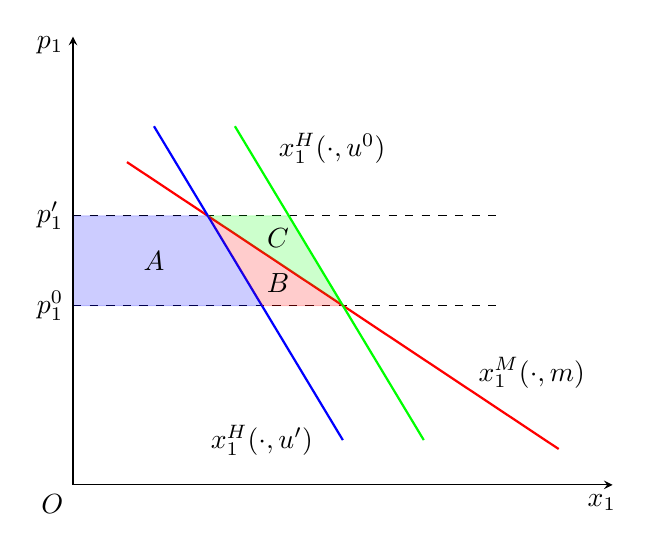
\begin{tikzpicture}
    \begin{axis}[
        xmin=0, xmax=10,
        ymin=0, ymax=10,
        axis lines=left,
        xtick=\empty,
        ytick=\empty,
        axis on top,
        clip=false,
        xlabel style={at={(rel axis cs:1,0)},anchor=north},
        ylabel style={at={(rel axis cs:0,1)},anchor=east},
    ]

    \node[below left] at (axis cs:0,0) {$O$};

    \addplot[mark=none, dashed] coordinates {(0,4) (8,4)};
    \addplot[mark=none, dashed] coordinates {(0,6) (8,6)};
    \node[left] at (axis cs:0,4) {$p_1^0$};
    \node[left] at (axis cs:0,6) {$p_1'$};

    \addplot[domain=1:9, red, thick] {8 - 0.8*x};
    \addplot[domain=1.5:5, blue, thick] {11 -2*x};
    \addplot[domain=3:6.5, green, thick] {14 - 2*x};

    \addplot[blue,fill=blue,opacity=0.2] coordinates {(0,4) (3.5,4)   (2.5,6) (0,6)};
    \addplot[red,fill=red,opacity=0.2] coordinates {(3.5,4) (5,4)   (2.5,6)};
    \addplot[green,fill=green,opacity=0.2] coordinates {(5,4) (4,6) (2.5,6)};

    \node[anchor=center] at (axis cs:1.5,5) {$A$};
    \node[anchor=center] at (axis cs:3.8,4.5) {$B$};
    \node[anchor=center] at (axis cs:3.8,5.5) {$C$};
    \node[anchor=center] at (axis cs:3.5,1) {$x_1^H(\cdot,u')$};
    \node[anchor=center] at (axis cs:4.8,7.5) {$x_1^H(\cdot,u^0)$};
    \node[anchor=center] at (axis cs:8.5,2.5) {$x_1^M(\cdot,m)$};
    \node[left] at (axis cs:0,9.8) {$p_1$};
    \node[below] at (axis cs:9.8,0) {$x_1$};
\end{axis}
\end{tikzpicture}
\end{center}
\end{minipage}
\hfill
\begin{minipage}{0.3\linewidth}
    \centering
    $$
\begin{cases}
-CV = A+B+C\\
-EV = A\\
-\Delta CS = A+B
\end{cases}
$$
\end{minipage}

\rmkb{
\begin{enumerate}

\item
  If the Marshallian demand curve is steeper than the Hicksian demand
  curve, it implies that the good is an inferior good. In the graph, the
  represented good is a normal good.
\item
  On any range where the good in question is either normal or inferior,
  then:
  \[\min\{CV,EV \}\le \Delta CS\le \max\{CV,EV \}.\]
  Notice that the two cases are not exhaustive. For example, a good may
  be normal good at some lower ranger of price, but reversed to inferior
  good at higher range of price.
\end{enumerate}
}

\ex{
Suppose a consumer has a locally non-satiated and strictly convex
preference relation on \(\RR_+^2\) that can be represented by a twice
continuously differentiable utility function \(u(x_1,x_2)\ge 0\).
Moreover, for \((p_1,p_2)\gg \0\) and \(u\ge 0\), the expenditure
function is given by:
\[e(p_1,p_2,u) = \frac{p_1p_2u^2}{p_1+p_2}\]
\begin{enumerate}

\item
  For \((p_1,p_2)\gg \0\) and \(u>0\), derive the Hicksian demand
  \(\x^H(p_1,p_2,u)\).
\item
  For \((p_1,p_2,m)\gg \0\), derive the Marshallian demand
  \(\x^M(p_1,p_2,m)\).
\item
  Now suppose \(p_2 = 1\) and \(m = 2\). Consider a price drop from
  \(p_1^0 = 2\) to \(p_1' = 1\). Calculate the compensating variation
  (\(CV\)), the equivalent variation (\(EV\)), and the change in
  consumer surplus (\(\Delta CS\)) of this price change.
\end{enumerate}
}

\sol{
\begin{enumerate}

\item
  By Shephard's Lemma,
  $$
\begin{aligned}
  x_1^H(p_1,p_2,u) = \frac{\partial e(p_1,p_2,u)}{\partial p_1} = \frac{p_2^2u^2}{(p_1+p_2)^2}\\
  x_2^H(p_1,p_2,u) = \frac{\partial e(p_1,p_2,u)}{\partial p_2} = \frac{p_1^2u^2}{(p_1+p_2)^2}\\
  \end{aligned}
$$
  It follows that
  \(\x^H(p_1,p_2,u) = \left(\frac{p_2^2u^2}{(p_1+p_2)^2},\frac{p_1^2u^2}{(p_1+p_2)^2} \right).\)
\item
  By duality,
  \[e(p_1,p_2,v(\p,m)) = \frac{p_1p_2v(\p,m)^2}{p_1+p_2} = m.\]
  We then have \(v(\p,m)^2 = \frac{p_1+p_2}{p_1p_2}m\).

  Again by duality,
  \[\x^M(p_1,p_2,m) = \x^H(p_1,p_2,v(\p,m)) = \left(\frac{p_2m}{p_1(p_1+p_2)},\frac{p_1m}{p_2(p_1+p_2)} \right).\]
\item
  Apply the definition of \(CV\), \(EV\) and \(\Delta CS\):
  $$
\begin{cases}
  CV = e(p_1^0,p_2,u^0)-e(p_1',p_2,u') = m-e(p_1',p_2,u^0)\\
  EV = e(p_1^0,p_2,u')-e(p_1^0,p_2,u') = e(p_1^0,p_2,u')-m\\
  \Delta CS = \int_1^2 x_1^M(p_1,p_2,m)\text dp_1 = 2\ln \frac43 = 0.58
  \end{cases}
$$
  Notice that \(u^0 = v(p_1^0,p_2,m) = \sqrt 3\) and
  \(u' = v(p_1',p_2,m) = 2\). Then the results are:
  $$
\begin{cases}
  CV = \frac12\\
  EV = \frac23\\
  \Delta CS = 2\ln \frac43\approx 0.58
  \end{cases}
$$
Note that typically we have $\min\brace{CV,EV}\le \Delta CS\le \max\brace{CV,EV}$. This can be used to double check the ``correctness" of your result.
\end{enumerate}
}

There is one thing noteworthy about aggregation. While we have laid the foundation for individually analyzing consumer's utility maximization problem, it may fail if we directly make the aggregation.

\ex{
Consider two consumers 1 and 2, whose preferences can be represented by
the following utility functions:
$$
\begin{aligned}
& u^1(x_1,x_2) = 
\begin{cases}
x_1x_2^3 & \text{if }0\le x_2\le 7.7\\
(7.7)^3x_1 & \text{if }x_2\ge 7.7\\
\end{cases}
\\
& u^2(x_1,x_2) = 
\begin{cases}
x_1^3x_2 & \text{if }x_1\ge 3x_2\\
\frac13 x_1^4 & \text{if } 0\le x_1\le 3x_2
\end{cases}
\end{aligned}
$$

Consider the following budget sets:
\begin{itemize}
\item
  Budget set \(A\): \(p_1 = p_2 = 2\), \(m = 20\).
\item
  Budget set \(B\): \(p_1 = 3\), \(p_2 = 1\), \(m = 20\).
\end{itemize}

Intuitively, the failure of aggregation is due to \emph{diverse income
effects}. For instance, in the example above, the price change has a
positive income effect on consumer 1, but a negative income effect on
consumer 2. Aggregation is possible in the special case where all
consumers have the same wealth effect, that is,
\(\frac{\partial \x^i}{\partial m^i}=\frac{\partial \x^j}{\partial m^j}\),
for every two consumers \(i,j\) and \(p,m^i,m^j\).
}

